\documentclass[aspectratio=169]{beamer}

\usepackage[russian]{babel}
\usepackage{amsfonts}
\usepackage{amsmath}
\usepackage{amssymb}
% \usepackage[cp1251]{inputenc}
\usepackage[utf8]{inputenc}
\usepackage{epigraph}
\usepackage{tikz}
\usepackage{xcolor}
\usepackage{verbatimbox}
\usepackage{pgfplots}
\pgfplotsset{width=10cm,height=6cm,compat=1.3}
\usepackage{multicol}
\usepgflibrary{arrows}




\usetheme{Madrid}

\newcommand{\SubItem}[1]{
    {\setlength\itemindent{15pt} \item[-] #1}
}

\newcommand*{\sele}[1]{{\bf #1}}
\newcommand*{\sel}[1]{\textcolor{blue}{#1}}
\newcommand*{\prob}[1]{\textcolor{magenta}{#1}}
\newcommand*{\vs}[0]{\vspace{10pt}}
\newcommand<>{\fullsizegraphic}[1]{
%  \begin{textblock*}{0cm}(-1cm,-3.78cm)
  \includegraphics[width={\paperwidth}]{#1}
%  \end{textblock*}
}

\title[Duplicates and SpellChecker]{Duplicates and SpellChecker}
\author{Pavel Ajtkulov}
\institute[]{ajtkulovp@dnb.com, Orb Intelligence / DnB}
\date{4 Jan 2021}

\begin{document}

\frame{\titlepage}



\frame
{
\frametitle{Duplicates}

{\huge Duplicates}

}


\frame
{
\frametitle{The Task}

\begin{minipage}{0.45\textwidth}
\begin{itemize}
  \item Profile \#1
  \item Name: Orb Intelligence
  \item Address1: 1900 Camden Ave
  \item City: San Jose
  \item State: California
  \item Country: US
  \item Zip code: 123456
\end{itemize}
\end{minipage}%
\pause
\hfill
\begin{minipage}{0.45\textwidth}
\begin{itemize}
  \item Profile \#2
  \item Name: Orb Intelligence Limited
  \item Address1: 1900 Camden St
  \item City: 
  \item State: CA
  \item Country: US
  \item Zip code: 123543
\end{itemize}
\end{minipage}%
}


\frame
{
\frametitle{The difference}

\begin{itemize}
\item Typos
\item missing data
\item changes (rename, moved to new address)
\item corporate elements (<<inc>>, <<limited>>)
\item normalization (<<CA>> / <<California>>)
\end{itemize}
}

\frame
{
\frametitle{The usage}

\begin{itemize}
\item The same company?
\item Looking for <<neighbours>>
\item Data cleaning, removing duplicates
\pause
\item Text/Item similarity (etc, legal pages, plagiarism detection)
\end{itemize}
}


\begin{frame}[fragile]
\frametitle{The method}

Locality Sensitive Hashing (LSH) - family of algorithms. 

\vspace{2mm}

Similar inputs $\rightarrow$ similar hashes.

\pause

\vspace{2mm}
For string input, hash is binary vector + Hamming Distance. 

\pause
\vspace{2mm}
On scale, it is the issue to traverse all similar hashes (we've solved it). 
\vspace{2mm}
\pause

\begin{verbatim}
001110101111100101 
001001011010101101 
       ...
111110011011010010 
001001111011100101 
000001100000011100 
\end{verbatim}

\pause
\begin{verbatim}
Request(001001011010101101) = 
  List[(001001011010101101, 0 Err), (001001011010101101, 3 Err)]
\end{verbatim}
\end{frame}

\frame{
  \frametitle{Adjustment - 1}

\begin{itemize}
  \item Name: The Washington Times
  \item Address1: 123 Washington Street
  \item City: Little Washington
  \item State: Washington
  \item Country: US
  \item Zip code: 925135
\end{itemize}

\pause

Sub-string <<Washington>> has different meanings.
}

\frame{
  \frametitle{Adjustment - 2}

Priorities. 

\begin{itemize}
  \item Name is more relevant
  \item Corp element could be ommited (less priority for comparison)
  \item Coutry/State consists of 2-3 chars after normalization
\end{itemize}

}

\begin{frame}[plain]
  \frametitle{Trie - 1}

      \begin{figure}
        
\includegraphics[height=0.4\textwidth]{trie1.png}
      \end{figure}
\end{frame}

\begin{frame}[plain]
  \frametitle{Trie - 2}

      \begin{figure}
        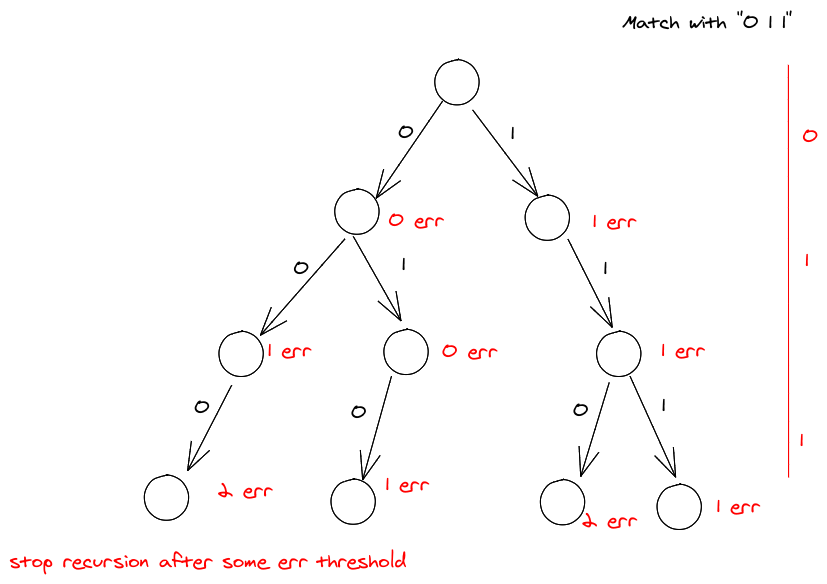
\includegraphics[height=0.4\textwidth]{trie2.png}
      \end{figure}
\end{frame}

\begin{frame}[plain]
  \frametitle{Trie - 3}

      \begin{figure}
        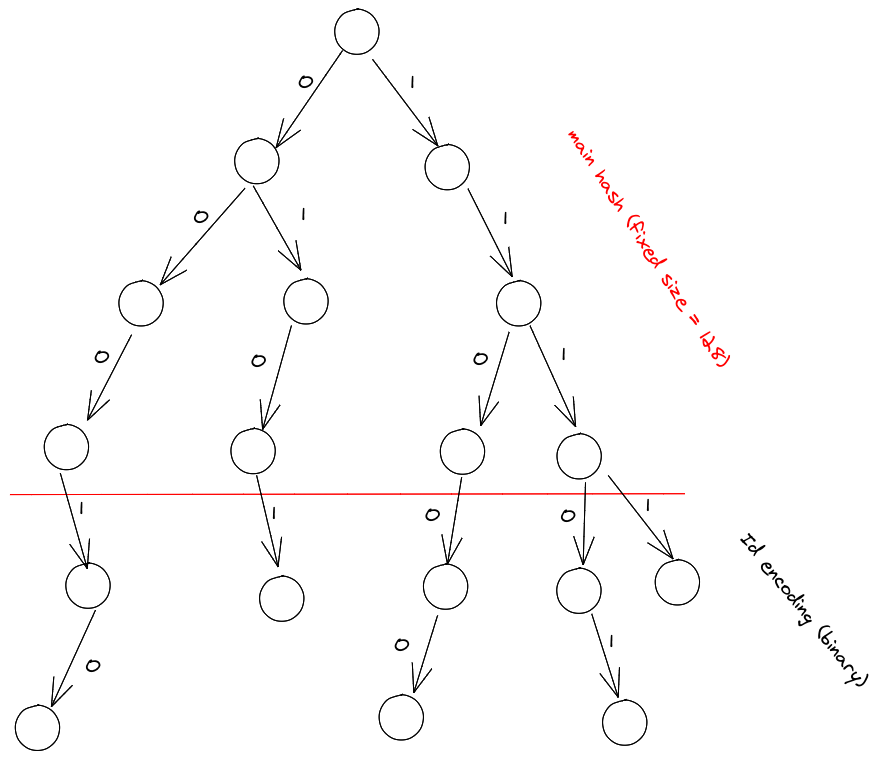
\includegraphics[height=0.4\textwidth]{trie3.png}
      \end{figure}
\end{frame}

\frame{
  \frametitle {The Flow}

\begin{itemize}

  \item Tear text (profile) into N-grams. {\color{blue} Use weight for priorities (new)}. {\color{blue} Use salt (new) \footnote {To separate (<<Washington>> in name/city/state/address)}}. We have set of N-grams. Hash it to Long's.

  \pause 
  \item Loop: $i \leftarrow  1\ldots 128$.
     Use random permutation for $0\ldots2^{64} - 1$ (mod p, generator, Number Theory). Select minimum hash of all N-grams after applying random permutation \footnote {Find minimum hash for random permutation == two text share the same n-gram}. Select lower bit \footnote{If they share the same n-gram, then bit is the same. Otherwise, equal with 50 per cent probability.}. So, we have 128-bit hash.
  \pause 

  \item Put all binary hash + ID (company profile ID) into trie \footnote{\color{blue}Trie implementation is Bloom Filter (boolean checks for prefix and final string). To reduce memory consumption (new).}.

  \pause
  \item To lookup with threshold error, no more than K-errors in Hamming Distance. Traverse trie with recursion.
\end{itemize}


}


\frame {
  \frametitle{The results - 1}

\begin{itemize}
  \item May, 2020
  \item GDMI data (360M+ profiles, actually 400M+ names, including name + DBA)
  \item RAM 20 Gb index
  \item Full scan. AWS, 5 days, 24 nodes, 72 vCPU (36 physical CPU), spot instances
  \item About \$3000

\end{itemize}

}

\frame {
  \frametitle{The results - 2}


}









\end{document}
